\chapter{Technical Background of TOF Lidar}
%%%%%%%%%%%%%%%
% laser source
%%%%%%%%%%%%%%%
\section{Fundamentals of Laser Source}
% 1. Type of laser
% laser source is the starting poing of a TOF laser, which provide laser. There are different kinds of laser: solid-state, edge-emitting, fiber .... overview of different laser is given in ref..., this work uses fiber laser. The benefit of fiber laser is long coherent length, can be focused on a small spot. 
% 2. Important parameters:
% (1)Peak power, average power, relation, to see long distance, need high peak power
% (2) wavelength, 905 vs 1550, eye safety(power limitation), detector (ref: section...), beam spot size
% (3) BW and rise time --> rise time ristime = 0.35/BW, why narrow beam
% (4) pulse width -> range resolution ??
% (5) PRF: <-> distance


%% Questions: effect of temporal coherence? 
% beam size, coherency,<-- read [laser system eng book]
Laser source is the heart of a lidar system, which provides laser pulses that are transmitted to the free space and be detected by photon-detectors. Laser sources can be divided to different categories according to the gain medium where simulated emission of photons and the optical gain takes place. Examples of different types of laser include semiconductor lasers, solid-state lasers, fiber lasers, and gas lasers \etc Different types of laser have their own characteristics and specific applications. For an overview of different laser sources readers could refer to \todo{add referece: laser system eng} and this work will focus on an introduction of the key parameters of a laser source, and discussion of the concerns of parameter selection for the application of a range-finder lidar. 
\subsection{Parameters}
Key characteristics of a laser source include temporal and spatial coherence, wavelength, pulse width, rise time, pulse repetition frequency(PRF), enegy and power \etc which will be illustrated individually next.
\subsubsection{Temporal and spatial coherence}
Temporal coherence of a laser source describes the average correlation period between two wavelengths over which they becomes completely out of phase. The temporal coherence can be specified by a \emph{coherent time} $\tau_c$ and the corresponding \emph{coherent length} $d_c=c\tau_c$:
\begin{equation}
\tau_c = \frac{1}{2c}\frac{\lambda_0^2}{|\Delta\lambda|}    
\end{equation}
where $c$ is the speed of light, $\lambda_0$ is the center wavelength of a laser and $\Delta\lambda$ is the \emph{linewidth} of a lase. The linewidth is the wavelength difference from the center wavelength in a laser spectrum, caused by gain medium, quantum-mechanical, and opto-mechanical broadenings of the wavelength, \etc The temporal coherence of a laser tells the degree of monochromatic of a laser, \ie a laser with larger linewidth starts to decorrelate faster. Low temporal coherent laser is more likely subject to \emph{chromatic aberration}, which is a fact that a lens is fail to focus all the wavelengths to a same convergence point. Specifically, if a laser has a wide spectrum, the beam could disperse after the focusing lens due to that a lens has different refractive indices for different wavelengths of light. Minimizing the chromatic aberration is important for a range-finder lidar, since large dispersion of the laser requires a large size of a detector which could introduce more unexpected ambient light.\todo{check the effect of temporal coherence on measurements} However, speckle noise is a drawback of a temporal-coherent laser, because the reflection of highly correlated beams from rough surfaces causes stable interference. The interference could produce obvious speckle patterns which affects the power of return pulses and the image quality of a flash lidar.\\
Spatial coherence describes the phase correlation across the wavefront of a laser beam. For a spatial coherent beam, the irradiance distribution profile is an ideal Gaussian profile. However, in practice, due to unavoidable misalignment between the mirrors of a laser cavity, the distribution profile (wavefront) becomes a near-Gaussian profile superposed by non-Gaussian beams which results in phase variation, and the laser becomes spatial incoherent. The degraded spatial coherence due to the phase distortion results in (1) an increase of divergence angle at which the beam exits the laser, and (2) an increase of the spot size when the beam is focused with a lens. Therefore, spatial coherent beams are also called diffraction-limited beams. The spatial coherence of a laser beam can be quantified by the beam quality factor $M^2$. Specifically, for a diffraction-limited beam the beam quality $M^2=1$, while for the beam that is not diffraction-limited, $M^2>1$. The spatial coherency is also crucial for a TOF lidar. One one hand, a large beam size due to large divergence of a beam at a long distance limits the resolvable size of a target and makes the edges less resolvable. A large beam size can also cause multiple-path effects~\citep{adams2000lidar}. On the other hand, when the return laser is focused on a detector, the increasing spot size requires a larger detector to cover the whole profile, which allows more background light incident on the detector and increases electrical noise of the system. However, similar to the temporal coherence, the speckle noise is also a disadvantage of a spatial-coherent laser. It is because the standard deviation of the speckle noise ~\citep{richmond2010direct}:
%% check the Dof and M2: sigma = i/sqrt(Dof)
\begin{equation} \label{eq:speckle}
\sigma_{sp}=\frac{i}{M}
\end{equation}
is largest compared to a diffracted laser for an ideal laser (\eg single longitudinal mode in time and single mode in space) that is temporal and spatial coherent (\ie $M^2=1$). The $i$ in Equation~\eqref{eq:speckle} is the signal current output from a photon-detector. Therefore, a laser with broadband spectrum and low spatial coherence is less subject to speckle noise.
%% wavelength
\subsubsection{Wavelength}
The wavelength is another important factor of a laser source. The most common wavelength bands for the TOF lidar application are near infrared band (NIR, $0.7-1.1\mu m$) and shortwave infrared band (SWIR, $1.1-3.0\mu m$). Two respective examples in the commercial for each band are $905 nm$ and $1550 nm$ with some variances \todo{add velodyne, luminar reference using different wavelength}. Each band of wavelength has its own advantages and weakness from different perspectives. ~\citep{wojtanowski2014comparison}\todo{change the way of citation} studied the vulnerability of the $905~nm$ and $1550~nm$ laser to different environmental conditions \wrt normal atmospheric conditions and conditions with high water content. The results show at normal atmospheric conditions, the atmospheric extinction coefficient for $1550~nm$ is two times lower than that for $905~nm$, while the water extinction coefficient for the former one is two orders of magnitude higher than latter one (show in Fig \todo{add water extinction coef fig, look at wojtanowski2014comparison}). The comparison indicates that $1550~nm$ could provide farther measurable distance at normal conditions, but at conditions with an increasing humidity, rains, fogs or wet targets, the maximum detectable distance for $1550~nm$ drops dramatically. Moreover, the water absorption of the wavelength is only a portion of the atmospheric effects on the laser. The other influence of the atmosphere on the laser include Mie-scattering of fog, specular reflection of rain droplets, and complex reflection mechanisms at a wet surface~\citep{wojtanowski2014comparison}, which will be briefly discussed in Section \todo{add section ..}.\\
In addition to the effect of atmosphere, the eye-safety of a laser is also needed to be considered when chose a wavelength. According to \todo{add eye safety reference} the maximum permissible exposure (MPE) for $905~nm$ is five orders lower than $1550~nm$ with an exposure time of $1~ns$ \todo{check with Sree about order and exposure time}. It is because $905 nm$ wavelength is close to the visible light range and can be focused to a tiny spot on the retina, while $1550~nm$ wavelength rarely reaches the retina due to high water absorption of the interior of human eyes and it is less hazardous. Therefore, the laser safety standards allow higher power output at $1550~nm$ which provide a positive impact on the maximum measurable distance.
The selection of wavelength is also depended on the requirement of photon-detectors, so the performance of detectors under different conditions also needs to be taken into account. More details of the behavior of detectors will be discussed in Section...\todo{add section of detector}. 
\subsubsection{Pulse width and rise time}
Another key parameter for a laser is the pulse width which is the time duration of a pulse, and is usually approximated by the Full width half maximum (FWHM) for a Gaussian pulse. For a TOF lidar, the pulse width indicates the illumination length of a target by a laser pulse, which determines the range resolution $\Delta R=c\Delta t_w/2$. Another parameter of importance is the rise time defined as the time required for a pulse to rise from 10\% to 90\% of its peak value. The relation between the rise time $t_r$ and the pulse width $\Delta t_w$ can be derived from Equation \eqref{eq:FWHM} and Equation \eqref{eq:rt} such as $ t_r\approx0.7164\Delta t_w$. The rise time of a laser pulse affects the timing accuracy of a TOF lidar which will be elaborated in Section \todo{add section}. The pulse width and rise time of a Gaussian pulse are shown in Fig \todo{add pulsefigure} as an example.
\subsubsection{Pulse repetition rate}
The pulse repetition rate $\mathit{PRF}$ is defined as the number of pulse transmitted by a laser source per second. The $\mathit{PRF}$ represents the number of product per second for a scanning lidar, and the frame rate for a flash lidar, assuming one image frame is generated from one flash of the source. In addition, the $\mathit{PRF}$ also limits the maximum achievable range of a laser: $R_{max}=c/2\mathit{PRF}$. An explanation is that, when a laser emits a first pulse, the timing device associates the returns with the first pulse only before the second pulse is emitted. When the second pulse is emitted, the returns from the first pulse will be considered as the returns of the second pulse. Therefore, there is a trade-off between the number of points per second and the maximum distance a lidar can achieve.
%% power and energy
\subsubsection{Power and Energy} \label{sec:pw}
Pulse energy $E$ is the power integration over the time duration of a pulse, and can be calculated using the pulse width and peak power for a rectangular pulse
\begin{equation} \label{eq:energy}
E=\int P(t)dt=P_0\cdot \Delta t_w.
\end{equation}
The pulse energy of a Gaussian pulse can also be approximated in the same under the assumption that the area under a Gaussian curve is equal to the area of a rectangular defined by the pulse width and the peak power, shown in \textcolor{red}{Fig, add figure1 in Budge}. Thus, a general form of the peak power of a pulse is derived as
\begin{equation}\label{eq:pw}
P_0=\frac{E}{\Delta t_w}.
\end{equation}
The peak power is a key parameter of a laser source, which represents the maximum optical power occurs during the pulse duration and significantly affects the maximum achievable range of a laser. In addition to the peak power, we also concern the average power of a laser which is defined as the power averaged over an entire period $T=1/\mathit{PRF}$:
\begin{equation}
P_{aveg}=\frac{E}{T}=E\cdot \mathit{PRF}.    
\end{equation}
The peak power and average power can be related by the \emph{duty cycle} of a pulse:
\begin{equation}
Duty~cycle= \frac{\Delta t_w}{T}=\frac{P_{aveg}}{P_0}    
\end{equation}


\subsection{Parameter selections for a TOF lidar}
%% suggestions: fiber: high spatial coherence, single mode, -->limited beam size, long distance due to small size, less energy diffusion. 
For a range-finder lidar, we would like to achieve a large maximum achievable range, a high resolvable angular resolution, large number of points per second and  ahigh measurement accuracy, which guides us on the parameter selection. Based on those considerations, we choose a single-longitudinal-model fiber laser as a laser source with a wavelength of $1550~nm$, a pulse width of $5~ns$ and peak power of $300~W$, and a $\mathit{PRF}$ of $1~\mathit{MHz}$. The reason for the selections are: 
\begin{enumerate}
    \item Fiber laser produces diffraction-limited beams which allows a smaller spot size at far distance (diameter $\approx 10~cm$ at 100 $m$ \textcolor{yellow}{sensl, 1mrad}) compared to diffracting laser. The small beam size leads to a high angular resolution and also increases the radiance (energy density). Fiber laser also allows a combination of short pulses width with high $\mathit{PRF}$ at high peak power~\citep{williams2017optimization}
    \item Narrow pulse width and fast rise time ensure high measurement resolution (0.75 $m$) and timing accuracy.
    \item High peak power allows longer maximum achievable range.
    \item The $\mathit{PRF}$ of $1 \mathit{MHz}$ balances the number of points (1 million points per second) and the maximum achievable range (150m).
\end{enumerate}

%%%%%%%%%%%%%%%
% Propgation
%%%%%%%%%%%%%%%
%%%%%%%%%%%%%%%
%% 2. Propagation
%%%%%%%%%%%%%%%
% propagatoin process: optics, atm, reflection  by targets, FOV

% (1) concepts
% Lidar Equation

% Start with Lidar equation, and divide to several sections:
% •	Optics parameters: transmission, FOV overlap, 
% (2) optic attenuation:lens transmission, optical filter, (why need it), FOV overlap, effect divergence of beam on power attenuation
% (3) Atmospheric effect: 
% o	fog model: visibility, wavelength
% o	effect of reflection by fog, rain: how the shape is changed, how the power is attenuated, effects on final distance (time delay due to multiple reflection)
% (4) Target properties: size (1/R2 or 1/R4), reflectively, geometry (angles)


\section{Radiometry of laser propagation}
This section discusses the calculation of laser power at each stage of the laser propagation. The propagation stages include the passage through optical lens, propagation though free-space, reflection by targets, and detection by a photon-detection. The optical power received by a photon-detector $P_r$ can be calculated from a generic Lidar equation:
\begin{equation} \label{eq:lidareq}
    P_r=L\cdot\frac{f(\rho)}{\pi}\cdot\Omega_r\cdot A_r\cdot\eta_{atm,\frac{R}{2}}\cdot\eta_{opt}\cdot\eta_{FOV}
\end{equation}
where $L$ is the laser radiance at a target distance $R$, $f(\rho)$ is the total reflectivity of the target which is function of reflectivity $\rho$ of the target material, $\pi$ in the denominator is to convert the radiance to irradiance assuming a lambersian reflection meaning the target has a diffusive reflection of the laser; $\Omega_r$ is the solid angle subtended to the laser receiver. $\eta_{atm,\frac{R}{2}}$ is the atmospheric attenuation of laser power with distance $R$, $\eta_{opt}$ is the overall energy loss due to the optics, and $\eta_{FOV}$ is the energy loss due to partial FOV overlap. Each parameter will be illustrated in the next.
% The radiometric quantities used in this work are introduced below.
% \paragraph{} is the emitted or received laser power per unit area, $W/m^2$.
% \textbf{Laser brightness or radiance} is the 
\subsubsection{Laser beam divergence}
Even though a fiber laser can produce diffraction-limited laser beam, the divergence angle exits the fiber is still too large ($\approx15^{\circ}$). The divergence can be reduced by using a collimator to the order of $1~mrad$, but a beam of size of $7~mm$ can still be enlarged to $\approx10~cm$ at a $100~m$. The extended beam size reduce the radiance of the laser at a long distance. Since the target size is unknown, it can not be ensure that the entire beam can be reflected by the target (\eg the target size is smaller than the beam size). Therefore, it is beneficial to calcualte the radiance of the laser beam at the target distance. If the attenuation of the atmosphere and the optics are skipped for now, the radiance of the laser beam at a distance $R$ can be found under the paraxial approximation
\begin{eqnarray}
    L=\frac{P_0}{A_b}\\
    A_b=\frac{\pi}{4}(2\theta_{div}R+D)^2
\end{eqnarray}
where $P_0$ is the power at the exit of the fiber, $A_b$ is the beam size at the distance $R$. The divergence angle of the beam after a collimator is $\theta_{div}$ and the diameter of the collimator is $D$.

%% target
\subsubsection{Reflection of targets}
The factors of a target that influences the laser power includes the target size, the angle between the normal of the target surface and the looking-angle of the receiver (assuming the target has a single flat surface), the geometry of the target (if the surface of the target is complex), the materials of the target, and reflection mechanism of target and the content (\eg water) above the surface, \etc\\
The effect of the target size, materials, and the angle can be taken into account when calculate the exitance of the laser reflected by the target

take about lambiertian reflection... 

target direction
geometry
materials --> type of reflection


[cal,,,] studeid the effet of target on the power




\subsubsection{Effects of atmospheric conditions}
% spekcle noise, background light
The environment condition also has effects on the propagation of the laser pulse. Fog could attenuates on laser power. \cite{kim2001comparison} calculated the attenuation coefficient $\alpha$ in the Lidar equation:
\begin{align*}
\sigma&=\frac{3.91}{V}(\frac{\lambda}{550 \mathit{nm}})^{-q}\\
q&=1.6	&	&V>50 \textrm{km}\\
&=1.3	 &	6 \textrm{km}<&V<50 \textrm{km}\\
&=0.16V + 0.34	&	1 \textrm{km}<&V<6 \textrm{km}\\
&=V-0.5	&	0.5 \textrm{km}<&V<1 \textrm{km}\\
&=0	&	&V<0.5 \textrm{km}\\
\end{align*}
where\begin{align*}
\sigma &=\textrm{attenuation coefficient of the atmosphere}, km^{-1}\\
V&=\textrm{visibility}, km\\
\lambda&=\textrm{wavelength}, nm\\
q&=\textrm{the size distribution of the scatting particles}
\end{align*}

\subsubsection{Effects of optics}



%%%%%%%%%%%%%%%
%% Detector
%%%%%%%%%%%%%%%
\section{Photon-detectors and System Noises}
% Definition of different noises, dark current, cause of different noise, distribution of the noise, white/not white
% difference betwen SI and InGaAs, 905 vs 1550, darkcurrent, band gap,  etc..
%5 bandwidth of a detector: rt = 0.35/BW, BW = RC...
% •	Shot noise: signal-, dark current-, background light-
% •	Calculate background noise
% •	F
% •	Thermal noise: APD and TIA
% Appendix: derivation of shot noise equation

\subsection{Fundamentals of photon-detectors}
what is a detector, different kinds: 
-different materials, si, ingaas, differences
what is tia
\subsection{System noises}
shot noise
thermal noise
system noises include noises from atm (background light), inherent noise 

%%%%%%%%%%%%%%%
%% Noise and Filter Module
% %%%%%%%%%%%%%%%
% Another classification of the noise: time domain, and frequency domain, structured/random noise
% fundamentals of filter (analog): important parameters (time and frequency domain). Characteristics of different filters: cheby, butterworth, etc.
% fundamentals of wavelet filters: parameters



\subsection{White noise and structured noise} \label{sec: noise}
% From atmosphere: 
% --turbulence, speckle
% -- ambient light
% --target surface

% Electrical noise:
% --shot noise
% --avalanche noise 
% --thermal noise

% When the photon detector of a lidar converts laser beams to electrical signal, noise is added to the returning signal as well. The noise can be generated from different sources, for example, ambient light or turbulence in the atmosphere, surface change of objects in the environment, parameter variation in the electrical system, etc. The source of the noise and their characteristics will be illustrated in this section.


%%\subsection{Type of Noise}
According the characteristics of the noise in time and frequency domain, the noises can be divided into three categories: white noise,  frequency-structured noise, and temporal-structured noise.\par
The white noise is the noise that has a constant power spectral density spreading all the frequencies. Both shot noises and thermal noises are white noise \cite{Kittel2004ElementaryPhysics}\cite{Blanter2000ShotConductors}, because their power spectral densities are independent on frequency $f$:
\begin{align}
S_{shot}(f) &= 2q\overline{I} \\
S_{thermal}(f) &= 4k_BRT
\end{align}
where $S$ is the power spectral density, $q$ is the electron charge, $\overline{I}$ is the signal average current over the detector integration time,  $k_B$ is the Boltzmann's constant, $R$ is the resistance, and $T$  is the overall temperature of the system. The difference between the shot noise and the thermal noise is that at each event the shot noise is Poisson distributed (\ie the magnitude of the noise is proportional to the signal magnitude), while the thermal noise has a Gaussian distribution which is independent on the signal amplitude. Therefore, the shot noise is Poisson-white noise and thermal noise is Gaussian-white noise. The variance of the noise can be obtained from: 
\begin{align}
\sigma_{shot}^2 &= 2q\overline{I}^2FB\\
\sigma_{thermal}^2 &= 4k_BRTB
\end{align}
where $F$ is the excess noise factor of an APD, and $B$ is the bandwidth of the system. An example of white noise is shown in Figure~\ref{fig:backgrd_Noise_white}.\par
Noises can also have certain structures in frequency domain which results from periodical appearance of the noise in time domain. Such noises are called frequency-structured noise in this study. The frequency-structured noise can be divided to in-band frequency-structured noise (IB-noise) and out-of-band noise (OOB-noise) depending on whether the noise frequency is within the bandwidth of the pulse signal. The frequency-structured noise can result from unclean power supply, impedance mismatch between the connections of electrical components, or periodic other noise source. An example of frequency-structured noise is given in Figure~\ref{fig:backgrd_Noise_frequency}, in which the noise oscillates with a frequency of 645MHz. \par
Contrary to the frequency-structured noise which has periodic occurrence, noise can also occur randomly in time domain, which is called temporal-structured noise. The temporal-structured noise usually have a certain shape in time domain, but its appearance is unpredictable. The temporal-structured noise could result from ambient light, reflection of laser pulse from surrounding objects except the target,  laser beams from other laser devices, and loss connection of cables etc. An example of the temporal-structured noise is shown in Figure~\ref{fig:backgrd_Noise_time}, in which the time-structured noise is overlapped with white noise. From the comparison with the power spectrum in Figure~\ref{fig:backgrd_Noise_white}, we can see the temporal-structured noise results in additional power inside the red region.
\begin{figure}[t!p]
\centering
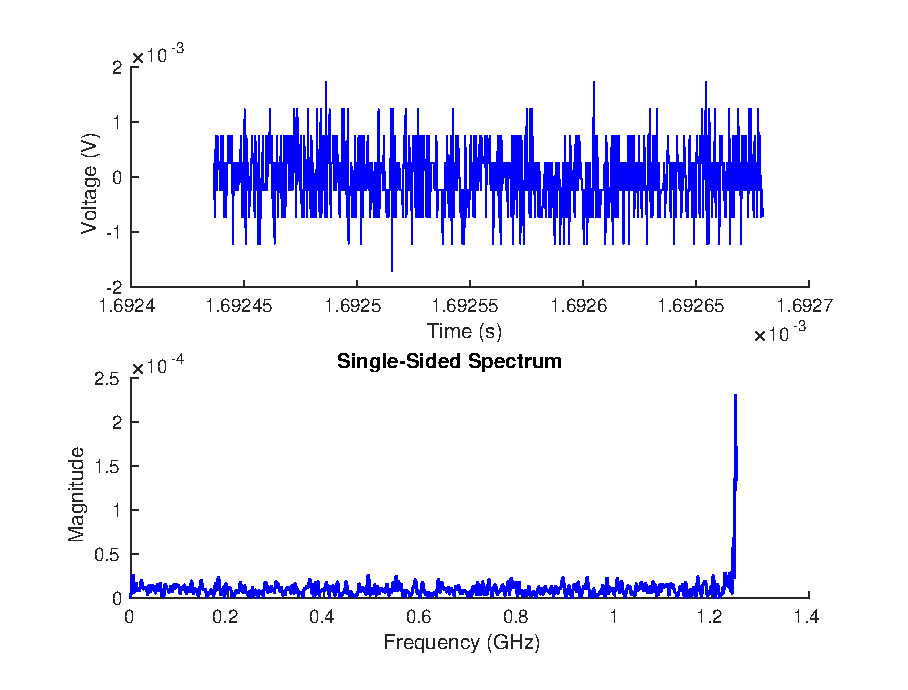
\includegraphics[width=.8\textwidth]{figures/chapter_background/Noise_white_sig_FFT_regWhiteNoise.eps}
\caption{White noise and its power spectrum}
\label{fig:backgrd_Noise_white}
\end{figure}
\begin{figure}[t!p]
\centering
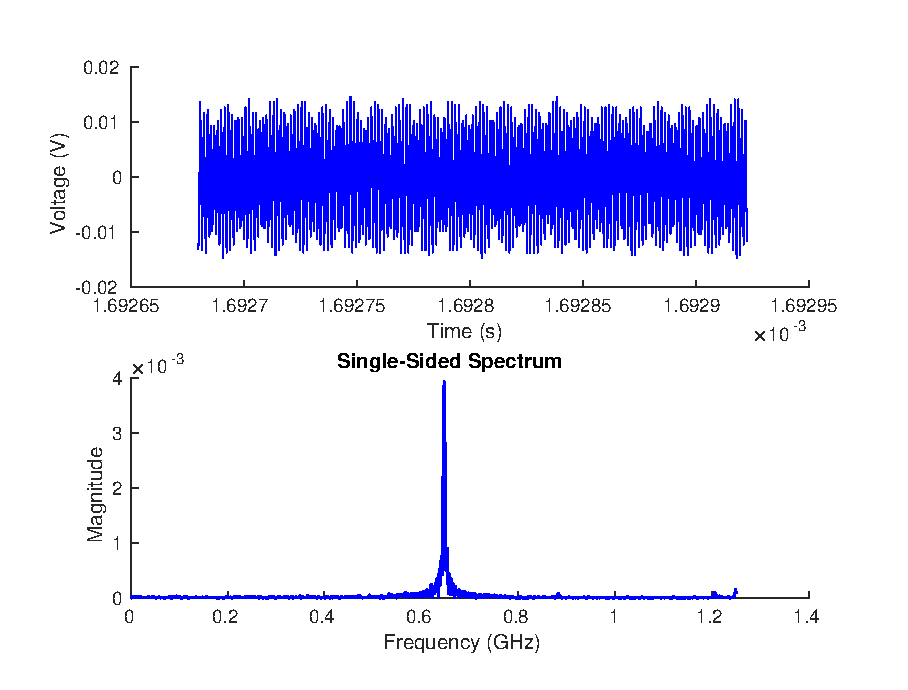
\includegraphics[width=.8\textwidth]{figures/chapter_background/Noise_freqStruct_sig_FFT_SineNoise2.eps}
\caption{Frequency-structured noise and its power spectrum.}
\label{fig:backgrd_Noise_frequency}
\end{figure}
\begin{figure}[t!p]
\centering
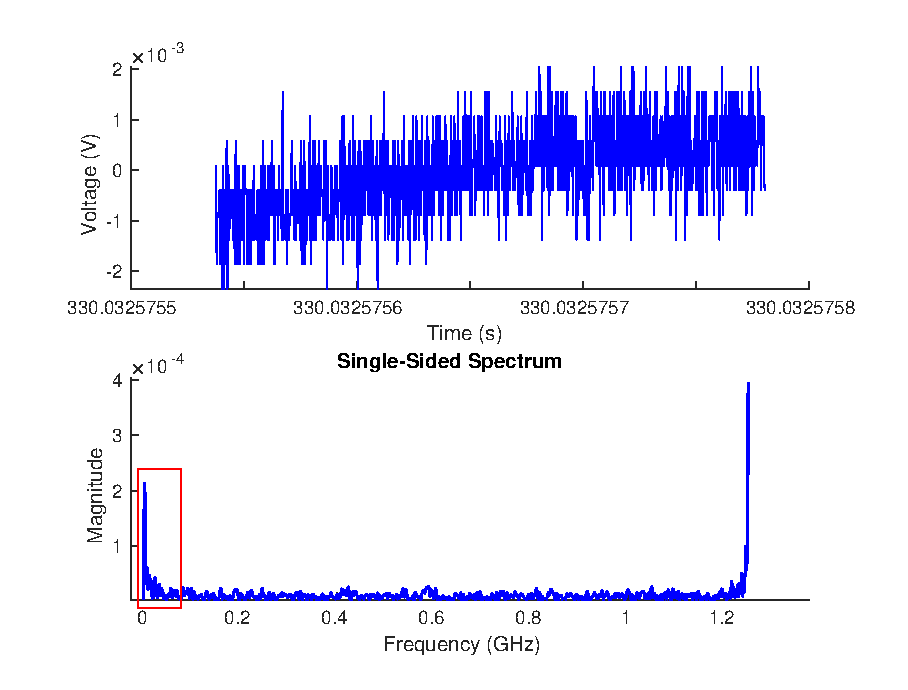
\includegraphics[width=.8\textwidth]{figures/chapter_background/Noise_timeStruct_sig_FFT_RampNoise.eps}
\caption{Time-structured noise. The noise in the red box is caused by the temporal-structured noise.}
\label{fig:backgrd_Noise_time}
\end{figure}

%%%%%
% Analog filter
%%%%%
\section{Filters}
In the application of laser rangefinder, the received laser pulse can be contaminated by all kinds of the noise mentioned above. The distortion of signals could result in uncertainty of the time measurement (Details will be described in Chapter~\ref{ch:TDC}, \ref{ch:ADC_BM} and \ref{ch:NP}). Therefore, the pulses need to be separated from the noise and should be restored if the signal is distorted. The noise removal can be achieved by filters. Filters have widely used in image processing, optics and electrical signal processing, and the filter referred to in this work is specifically for electrical signal processing. Generally, electrical filters can be classified as analog or digital filters. The simplest analog filters are RLC filters which are composed of capacitors, inductors and resistors, and other analog filters include crystal filters, microwave filters and mechanical filters \etc. The analog filters act on continuous-time (analog) signals, on the contrary, digital filters require an ADC to convert analog signals to digital samples, and processes digital signals by algorithms programmed in a digital signal processor (DSP). The section focuses on the fundamental concepts and characteristics of electrical filters but does not elaborate the details. Readers could refer to any textbook on signal processing for further information. The characteristics of electrical filters can be described in time and frequency domain. The characteristics in frequency domain is introduced first, followed by the time-domain characteristics.
% \todo{IIR and FIR? how do model }
\subsection{Frequency-domain Characteristics}
The characteristics in frequency domain of electrical filters can be described in time and frequency domain. sists of magnitude response and phase response. Figure~\ref{fig:Filter_freqResponse} presents a schematic of the frequency response of a low pass filter. The magnitude response describes the magnitude change (gain) by the filter at each frequency and the phase response presents the phase shift (or phase delay) at each frequency. The frequency response of a filter can be divided into three regions: \emph{passband}, \emph{transition band} and \emph{stopband}. The passband is the range of the frequencies passed by the filter, the stopband refers to the frequencies that are blocked, and the region in between is the transition band. According to the position of the passband at the frequency range, filters could be classified as low-pass (LP) filters, high-pass (HP) filters, band-pass (BP) filter, band-stop (BS) filters, and all-pass (AP) filters. The passband is bounded by a \emph{cutoff frequency}, $f_{cut}$, defined to be where the frequency magnitude response is reduced to -3 dB. In the passband, the frequencies are desired to be unaltered (flat passband or unity gain), but the gain may vary in certain filter designs and the fluctuation is called \emph{passband ripple}. Since large passband ripples alter the magnitude of in-band frequency components, the passband ripple should be remain small in a filter design. In the stopband, the blocked frequencies are attenuated by a \emph{stopband attenuation} which is measured between the peak of the passband magnitude and the largest stopband lobe magnitude. To sufficiently attenuate the stopband frequencies, the stopband attenuation should be adequately large. Note that filters usually have different gains at passband and stopband, but the all-pass filter, as indicated by the name, passes all the frequencies with a unity gain. It seems the all-pass filter has no change on the magnitude of the signal, but it plays an important role of modifying the phase of the signal which will be described in the next section. \par
The \emph{roll-off} of a filter is another important concept which defines the \emph{steepness} or slope of the magnitude response in the transition band, and it also sets the corn frequency of the stopband. A fast roll-off is preferred for a filter to truncate the undesired frequency band without affecting the rest spectrum, but the cost is the distortion of the frequency components at the passband. In other words, a steep transition band and a flat passband can not be achieve at the same time. Another key characteristic of a filter is the \emph{order}. The order of a filter is defined as the highest exponent in the numerator or denominator of the transfer function. The concept of the transfer function will not be expanded in this work, but in general, the order of a filter is equal to the number of delay elements in the filter structure, meaning that a filter of a large order offers a better magnitude response, but the large order also increases the complexity of the structure.
\begin{figure}[t!p]
\centering
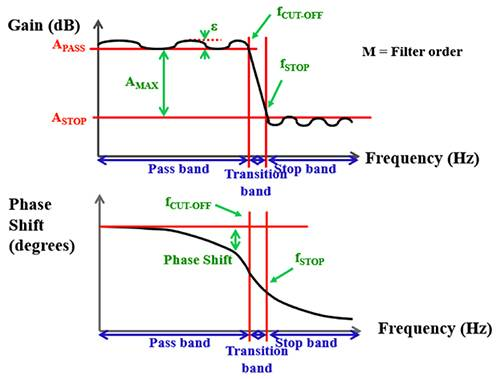
\includegraphics[width=.8\textwidth]{figures/chapter_background/Filter_freqResponse.jpg}
\caption{Frequency response of a low pass filter: (a)Magnitude response (b) Phase response}
\label{fig:Filter_freqResponse}
\end{figure}
\subsection{Time-domain Characteristics}
In addition to the frequency-domain characteristics, the performance of a filter in time domain is also important, and the step response of a filter is a useful tool for the analysis of a filter in time domain. The time-domain parameters include the \emph{rise time} and \emph{overshoot} of the step response. The rise time of a filter describes the transition period of the step response, which should be short than the duration of a signal event (\eg changing from 'low' to 'high'), so that the event can be distinguished from the step response. Second, overshoot changes the magnitude of a signal, so it should be avoided when a filter is designed. Moreover, the phase response of a filter also plays a significant role in the time-domain characteristics of a filter. One of the key concept is the \emph{group delay} defined as
\begin{equation}\label{eq:backgrnd_AFE_groupDelay}
    \tau_g= -\frac{d\Phi(\omega)}{d\omega}
\end{equation}
where $\Phi(\omega)$ is the phase response at angular frequency $\omega$ and $\omega = 2\pi f$. The group delay is the slope of the phase response which depicts the linearity of the phase response. Here, the group delay should not be confused with the phase delay which is another key concept commonly used in the phase response. The phase delay is defined as following
\begin{equation}\label{eq:backgrnd_AFE_phaseDelay}
	\tau_{\Phi}= -\frac{\Phi(\omega)}{\omega}
\end{equation}
and it only describes the absolute phase shift at each frequency without any description of the relationship between the adjacent frequencies like the group delay does. Using Fourier transformation, a signal can be decomposed into several sinusoidal components with different frequencies. If a filter has a linear phase response, all the frequency components are delayed by the same phase, in which case all the components can still reconstruct the original signal shape, but only the time is shift. In this case, the phase delay is equal to the group delay. However, in the case of nonlinear phase response, the frequency components are shift by different amounts, so they can no longer compose the original signal shape, \ie the signal is distorted. If symmetric signals are used as in our case, the symmetry of the signal is impacted. Therefore, the linearity of the phase response is a powerful indicator of the distortion enforced by the filter, and a linear-phase filter is preferred for the applications that requires preservation of signal shapes. Additionally, the all-pass filter can also be used to alter the phase shift in this case. Even though the all-pass filter has no effect on the signal amplitude, it is designed to have different phase shifts among various frequencies, so that it can be placed after the other filters in the system to compensate the undesired phase shifts.\par
\subsection{Characteristics of different filters}
According to the characteristics of a filter in time and frequency domain, the filters can be designed in various types. The most common types of filter are Butterworth filter, Chebyshev filter, Elliptic filter and Bessel filter. The frequency response of the filters is shown in Figure~\ref{fig:Filter_freqResponse_diffType}. The magnitude response shows that both Butterworth and Bessel filter has no ripple at the passband, but the roll-off is slower than the other two. On the contrary, the Chebyshev and Elliptic filters sacrifice the flatness of the passband to achieve a faster roll-off, which is why they are commonly used for noise band removal. In the phase response, the Bessel filter has a maximally linear phase response, followed by the Butterworth filter having a a reasonable nonlinear phase response, while the phase response of the Chebyshev and Elliptic filters are very nonlinear. Therefore, the Bessel filter is the best option for the application where the shape of the filtered signal is crucial, and the shape distortion needs to be considered when the last two types of filter are selected. The application of the Butterworth, Chebyshev and Elliptic filters to different types of noise mentioned in Section~\ref{sec: noise} will be discussed in Chapter~\ref{ch:AFE}. 
\begin{figure}[t!p]
\centering
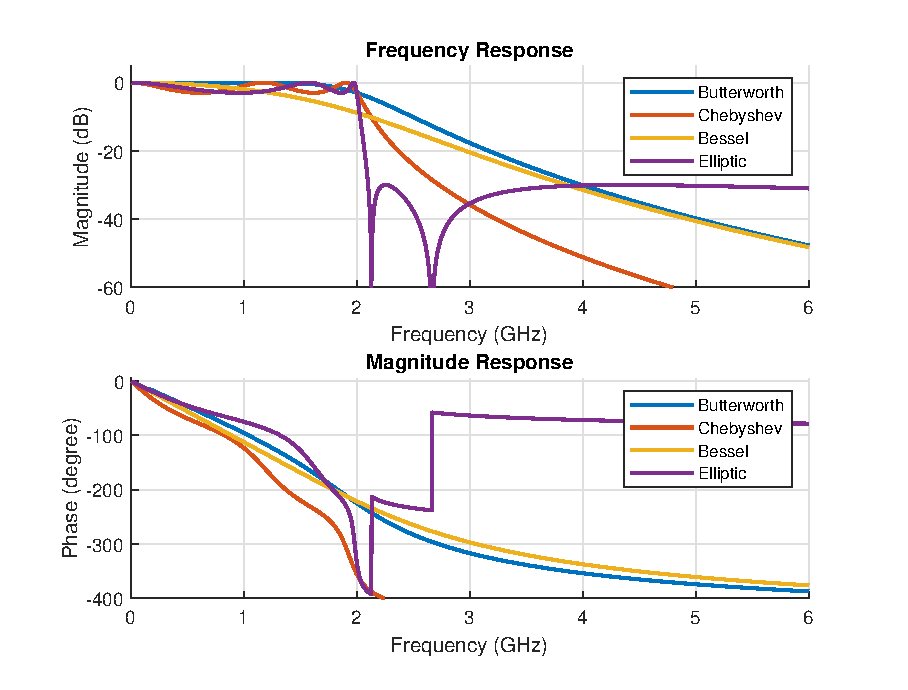
\includegraphics[width=.8\textwidth]{figures/chapter_background/Filter_FreqResp_diffFilters.eps}
\caption{Frequency response of different type of filters. The cutoff frequency is 2GHz, the order is 5, the passband ripple for the Chebyshev and Elliptic filter are 3 dB and the stopband ripple of the Elliptic filter is 30 dB.}
\label{fig:Filter_freqResponse_diffType}
\end{figure}
%%
% TDC
%%
\section{Time-to-Digital Converter}
After the photon detector converts returning laser pulses to analog signals, a time discriminator is required to measure the returning (stop) time of the signal. Given the transmitted (start) time of the pulse is measured beforehand, by calculating the time difference between the returning time and start time, the time-of-flight (TOF) of the emitted pulse and the corresponding distance of objects can be obtained. Generally, the start time and the returning time are usually discriminated by same techniques. Therefore, this section will only focus on the time discrimination techniques for the returning time, and the same principle is applied to the start time.\par 
Two approaches are commonly used for the time measurements. The first one is using a Time-to-Digital Converter (TDC), which consists of a comparator that generates logic signals by comparing input analog signals with a preset threshold, and a reference clock counter which measures the time when the logic signal changes its value from low to high. Both the start and stop time are measured in the same way. Then, the counter in the TDC subtracts the start time from the stop time to calculate the TOF. Different types of comparator and timing techniques will be described in the following sections, and Figure \ref{fig:TDC_schematic} presents a schematic of the TDC. The second approach is using an Analog-to-Digital Converter(ADC), which converts analog signals to digital signals. The ADC output is subsequently passed to a digital processor which performs numerical computation and extracts the time information of the signal. The TDC-based approach will be described next followed by the ADC-based techniques.\par
\begin{figure}[t!p]
\centering
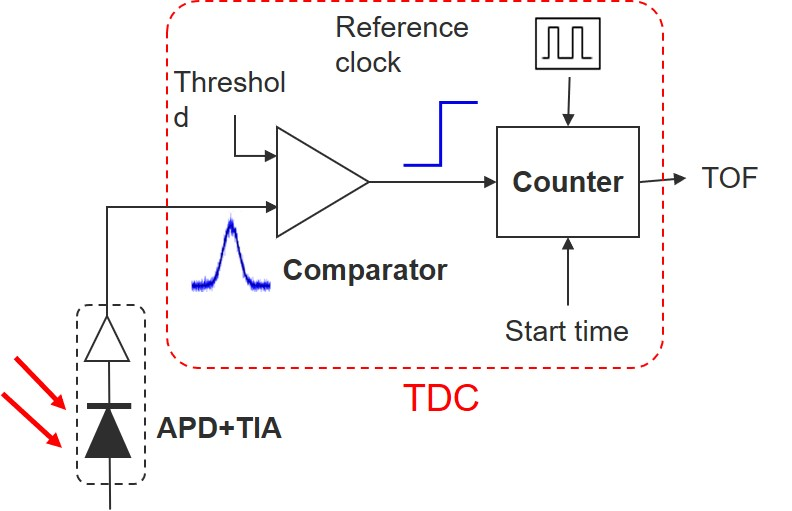
\includegraphics[width=.8\textwidth]{figures/chapter3_TDC/schematic_TDC.jpg}
\caption{Schematic of TDC}
\label{fig:TDC_schematic}
\end{figure}
Various time discrimination methods are available for the TDC-based approach. Generally, the discrimination techniques fall into two main categories: leading-edge discrimination and constant fraction discrimination (CFD). In this section, the leading-edge discrimination techniques will be introduced first followed by the CFD techniques.\par
% leading edge detection
\subsection{Leading edge detection}
In the leading-edge discrimination, time is measured when the leading edge of a signal crosses a threshold set at the comparator. Since the measurement is carried out at the leading edge of a signal, the time detection will still be functional even the signal saturates photon detector. In other words, the leading-edge detection is not restrained by the dynamic range of the detector. \par
However, the major disadvantage of the leading-edge discrimination is that significant the walk error could be introduced due to the variation of amplitude of the signal. The walk error is illustrated in Figure \ref{fig:TDC_walkerror}. In Figure \ref{fig:TDC_walkerror}, the two signals are reflected by the same target but have different amplitudes. Keeping comparator thresholds and rise-times of the signals the same, the signal with a smaller amplitude crosses the threshold later than the larger pulse. The time shift due to the amplitude change is called walk error. The walk error is a major concern for the leading-edge detection, which could lead to significant timing inaccuracy. Therefore, many methods have been developed to compensate for the walk error.
\begin{figure}[t!p]
\centering
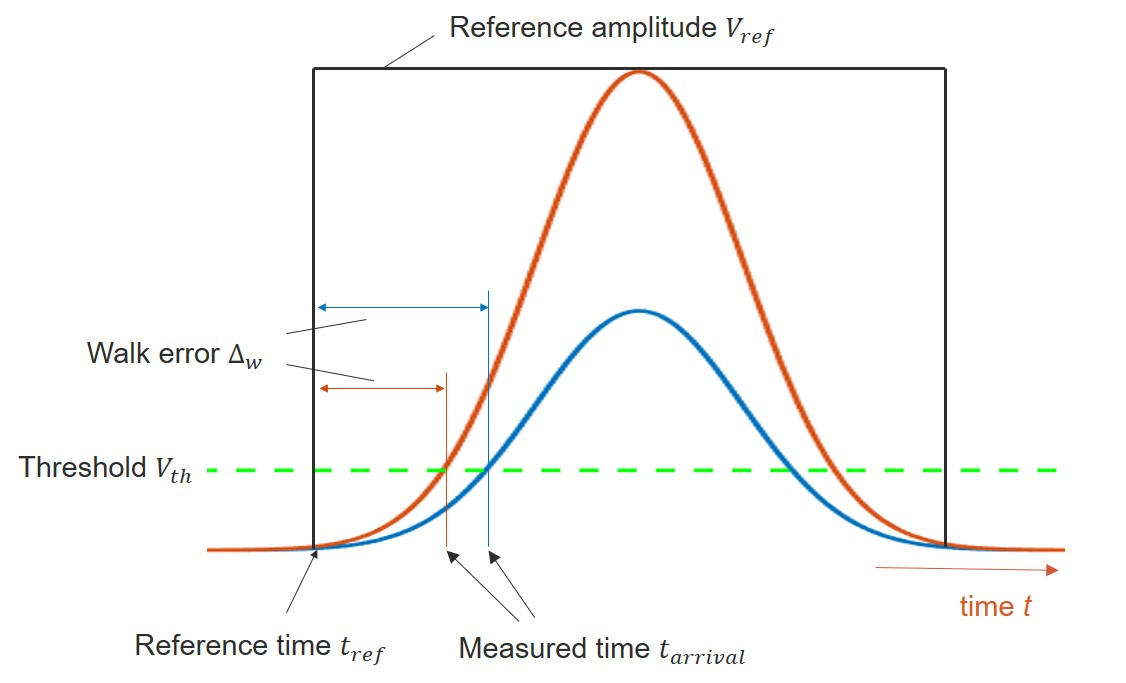
\includegraphics[width=.8\textwidth]{figures/chapter3_TDC/walk_error.jpg}
\caption{Illustration of walk error}
\label{fig:TDC_walkerror}
\end{figure}
%  insert TDC figure
\subsubsection{Gain-control compensation}
One way to reduce the walk error is to reduce the variation of signal amplitude by means of gain control. \cite{ruotsalainen2001wide} proposed a variable-gain amplifier followed by an amplitude-insensitive time discriminator. In the gain amplifier, the amplitude of a signal is first measured with a peak detector. Then, the attenuation of the gain control cells are adjusted accordingly to attenuate the amplitude of the signal to a constant value. Ideally, the gain-control technique allows a constant amplitude of a signal before entering the comparator. In practice, due to the limitation of the analog system, the achievable timing accuracy is $\pm 25 ps$ and the functional dynamic range is limited to $1:650$ \citep{ruotsalainen2001wide}. The limited operative range makes the gain-control less practical for the autonomous vehicle application, since the attenuation of the atmosphere and the reflectivity of the object can vary dramatically, which can result in a dynamic range of the amplitude of the signal of more than $1: 100,000$. 

\subsubsection{Time-over-Threshold (TOT) Compensation}
To allow a high dynamic range of input signals, the time-over-threshold(TOT) compensation and a slew-rate compensation were developed, \citep{kurtti2009pulse}, \citep{kurtti2011integrated} and \citep{nissinen2009integrated}. A schematic of the TOT compensation is shown in Figure \ref{fig:TDC_TOT}. In the TOT compensation, the crossing time at both leading edge and falling edge of a pulse are discriminated by the same comparator with the same threshold $Vth$. The time difference between the time marks at the leading and the falling edges is named the time-over-threshold (The time difference is named ‘pulse length’ in the original paper, but time-over-threshold is used here to avoid the confusion with the pulse width). As seen in Figure \ref{fig:TDC_TOT}, the TOT increases monotonically with the pulse amplitude and the walk error $\Delta_w$ decreases with the amplitude. Therefore, if the relation among the amplitude, walk error and the TOT can be found, the walk error can be determined and compensated by measuring the TOT.\par
\begin{figure}[t!p]
\centering
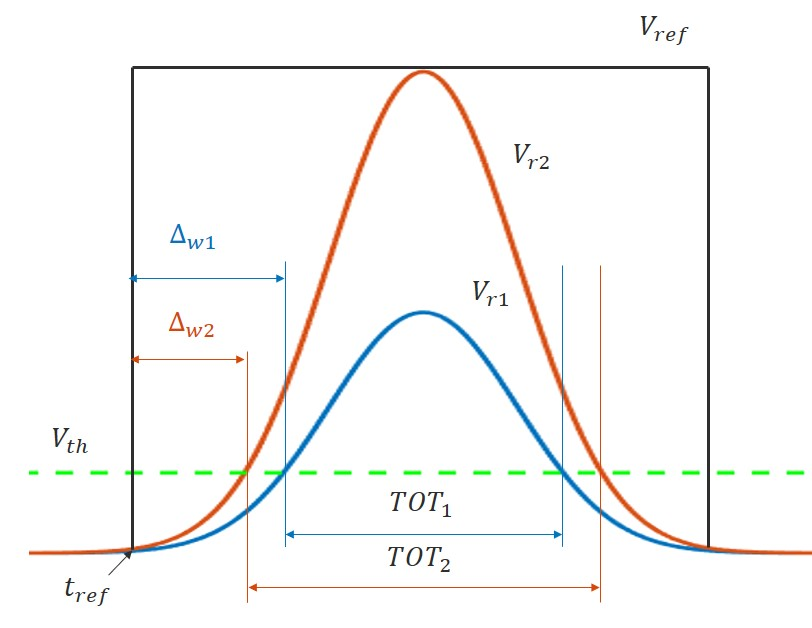
\includegraphics[width=.8\textwidth]{figures/chapter3_TDC/TOT.jpg}
\caption{Illustration of TOT compensation}
\label{fig:TDC_TOT}
\end{figure}
In practice, a look-up table or a compensation curve containing the relation of the walk error and the TOT is made by calibrating the TDC. It can be done by experimenting laser pulses with an amplitudes of a range of $1:100,000$, measuring the TOTs and walk errors for each amplitude, and calculating the corresponding ensemble average of TOT and walk error over the measurements. After the relation of the TOT and walk error is obtained, the walk error for a certain TOT can be found by extrapolating the compensation curve or the look-up table using the measured TOT value. Then, the walk error can be subtracted from the marked time at the leading edge of the signal to obtain the walk-error-free stop time. \citep{kurtti2009pulse} and \citep{kurtti2011integrated} proposed a compensation circuit to realize the TOT compensation. In this work, we provide the analytic relation among the TOT, pulse amplitude and walk error (The derivation is given in Appendix.): 
\begin{align}
    V_r&=\frac{V_{th}}{exp\big(\frac{(TOT/2)^2}{2\sigma^2}\big)}\\
    \Delta_w&=|t_{ref}|-\sqrt{t_{ref}^2-2\sigma^2\ln(\frac{V_{ref}}{V_r})}
\end{align}
where $V_{th}$ is the threshold, $V_r$ is the amplitude of a returning signal, sigma is the standard deviation of the signal, $t_{ref}$ and $V_{ref}$ are the convenient reference amplitude and time for calculation of walk error $\Delta_w$, and TOT is the measured TOT value. The relations between amplitude and TOT, amplitude and walk, and TOT and amplitude are presented in Figure \ref{fig:TDC_TOTcurve}. We also provide an analytic model of the TOT compensation process taking the TOT measurement as input and using the above relations. A schematic of the compensation process is shown in Figure \ref{fig:TDC_TOTcurve} (c).\par
The TOT method can achieve a time measurement precision of picosecond level and is operative in a larger dynamic range of the signal amplitude of $1: 30,000$ \citep{Kurtti2009PulseRangefinder}. However, we should notice that the TOT method is highly sensitive to the symmetricity of the signal. In other words, if the falling edge of the signal is heavily distorted due to, for example, multiple returns or amplification noise of the TIA, the relation between the TOT and the walk error is impaired. In this case, the TOT compensation will not be useful. 
\begin{figure}[t!p]
\centering
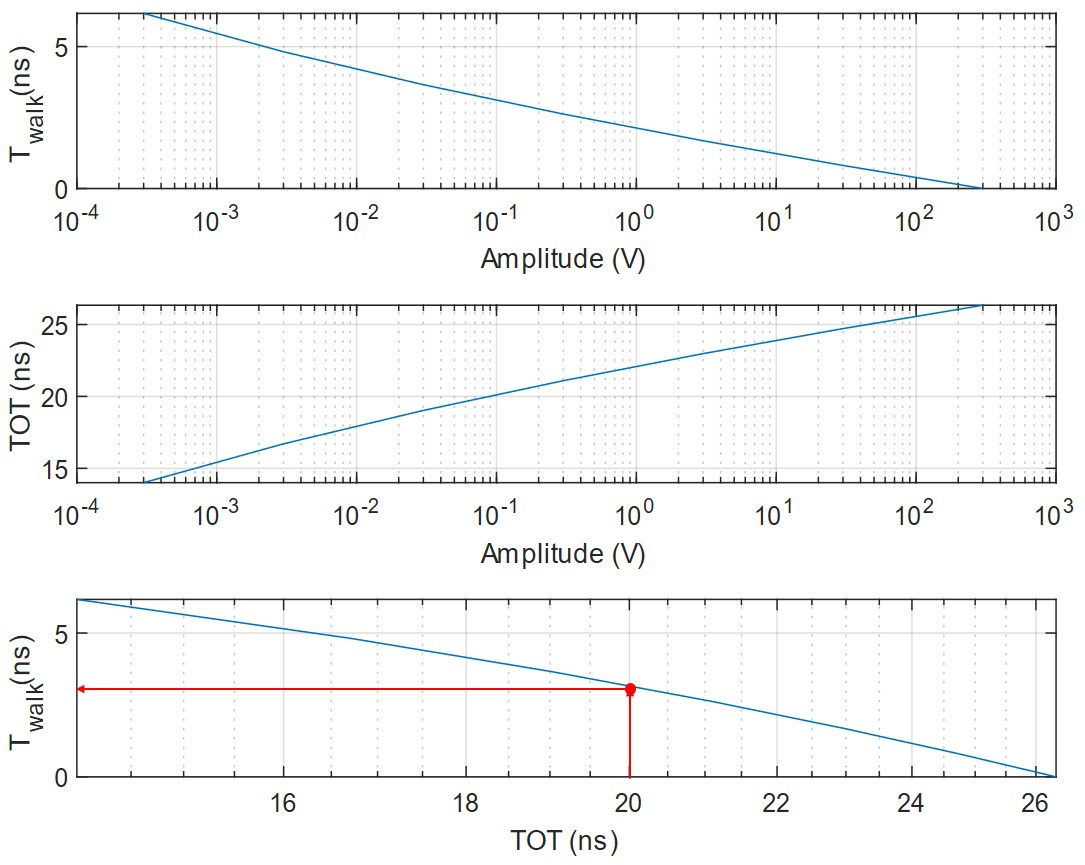
\includegraphics[width=1\textwidth]{figures/chapter3_TDC/TOT_curve.jpg}
\caption{TOT compensation curve}
\label{fig:TDC_TOTcurve}
\end{figure}
% slew rate
\subsubsection{Slew-rate Compensation}
An alternative way to compensate the walk error is to use the relation of the walk error and the slew rate of the return pulse, which is called slew-rate compensation. The slew rate is the slope of a signal at the point of interest. For the slew-rate compensation, the TDC is equipped with two comparators with two preset thresholds. A schematic of the slew-rate compensation is shown in Figure \ref{fig:TDC_slewrateLinear}\todo{change figure to sufigure and caption}. The lower threshold ($V_{th1}$) is set as normal in a TDC, and the higher threshold ($V_{th2}$) is set certain times larger than Vth1, i.e. $V_{th2} = CV_{th1}$. Two timestamps, t1 and t2 are measured from the comparator with respect to $V_{th1}$ and $V_{th2}$, and the time difference between $t_1$ and $t_2$, $\Delta_t$, is calculated. The walk error $\Delta_w$ is the time difference between $t_1$ and a convenient time reference $t_{ref}$. If the portions of the signal below the high threshold have a linear slew rate as shown in Figure \ref{fig:TDC_slewrate}, the walk error has a linear relation with the $\Delta_t$ \citep{nissinen2009integrated}:
\begin{align}
    \Delta_w=\frac{\Delta_t}{C-1}
\end{align}
\begin{figure}[t!p]
\centering
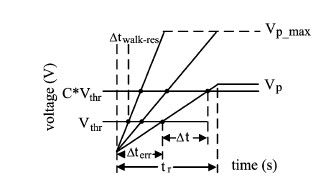
\includegraphics[width=.8\textwidth]{figures/chapter3_TDC/slew-rate.jpg}
\caption{Illustration of slew-rate compensation(linear)}
\label{fig:TDC_slewrateLinear}
\end{figure}
\begin{figure}[t!p]
\centering
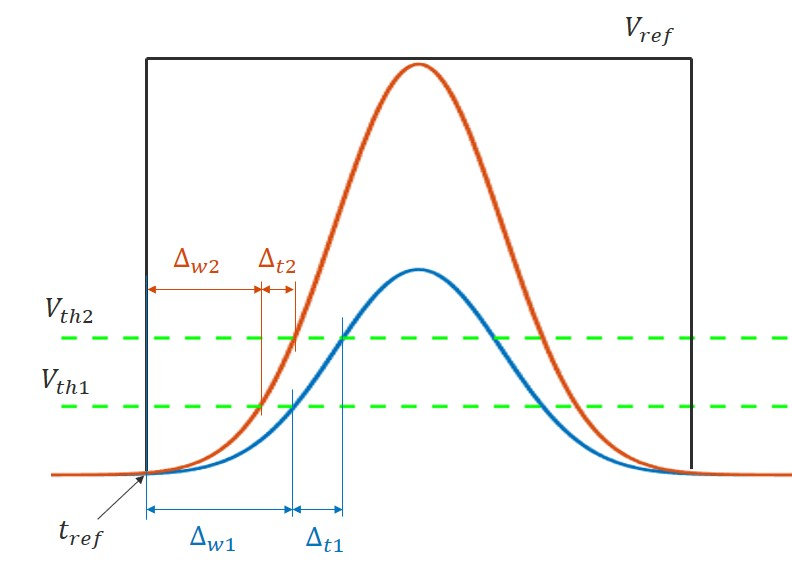
\includegraphics[width=.8\textwidth]{figures/chapter3_TDC/slew-rate0.jpg}
\caption{Illustration of nonlinear slew-rate compensation}
\label{fig:TDC_slewrate}
\end{figure}
However, a Gaussian signal usually has a nonlinear slew rate at the bottom, which results in a nonlinear dependency of the walk error on the time difference. Therefore, the dependency can be either obtained by calibrating the TDC like the TOT compensation or derived mathematically. For the calibration of the compensation curve or the look-up table, the walk errors and dts are first measured and calculated from signals with a wide range of amplitude, then, the averaged walk error and time difference is calculated for each amplitude. Consequently, the walk error can be obtained by extrapolating the compensation curve or the look-up table for a measured time difference, and the walk error is subtracted from the first stop time to remove the walk error on the return time.\par
In this work, we mathematically derived the nonlinear relation of walk error and time difference, and provide an analytical compensation model using MATLAB. The relationship is given as following and the derivation is detailed in Appendix. The relation between the walk error and the dt is plotted in Figure \ref{fig:TDC_slewrate_curve}.
\begin{align}
    \Delta_t&=STOP_2-STOP_1\\
    \Delta_w&=\frac{-2\sigma^2\ln(C)-\Delta_t}{2\Delta_t}-t_{ref}
\end{align}
\begin{figure}[t!p]
\centering
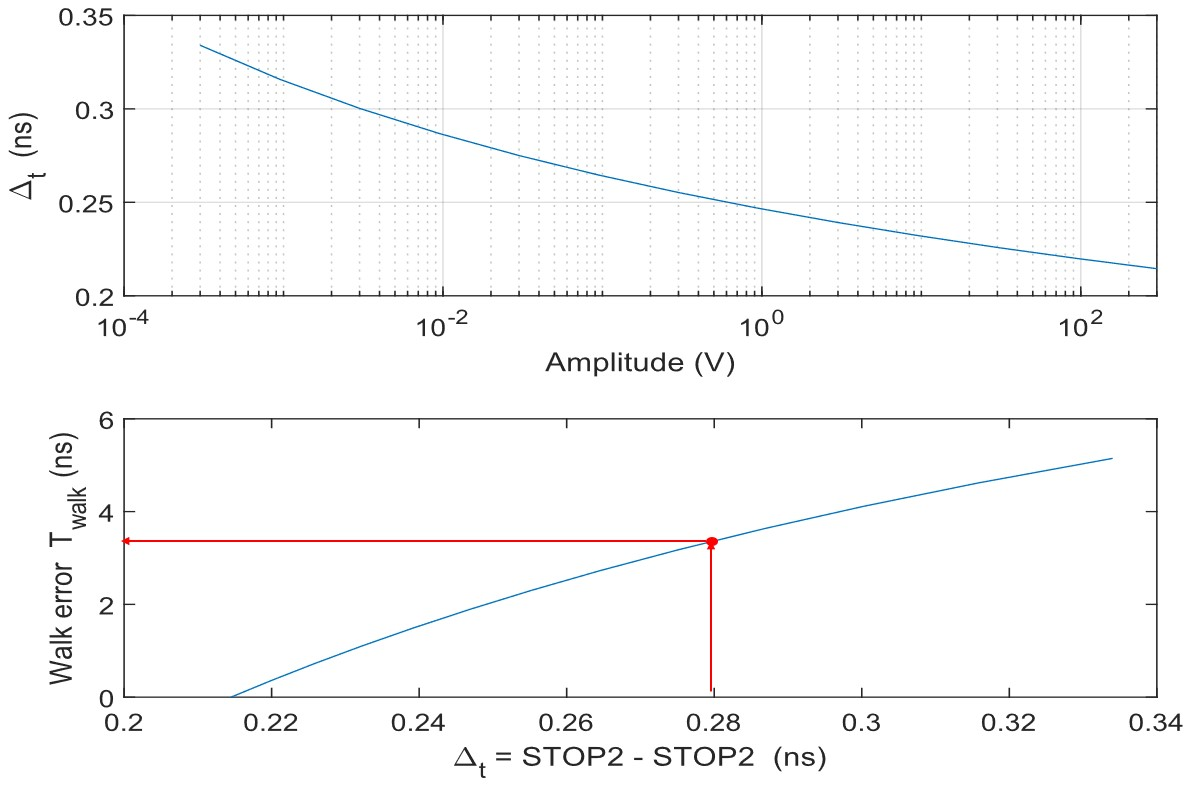
\includegraphics[width=1\textwidth]{figures/chapter3_TDC/slew-rate_curve.jpg}
\caption{Slew-rate compensation curve}
\label{fig:TDC_slewrate_curve}
\end{figure}
The slew-rate compensation can also achieve picosecond-level precision in large dynamic range as demonstrated by Nissinen. In addition, its independence on the falling edge of the signal makes it more applicable than the TOT compensation, but the additional comparator for the time difference measurement increases the complexity of the discriminator. \par
The TOT and slew-rate compensation significantly reduce the walk error, but also introduce additional noise to timing results. One example is the quantization error due to the utilization of extrapolation on the compensation curves, and the number of points used in the extrapolation affects the significance of the quantization error. In addition to the error induced by the compensation, the TDC-based timing techniques have their own inherent noises, of which jitter is an important one. Jitter is the uncertainty on measuring the time when a signal crosses the comparator threshold. If the signal is noise-free, the jitter on the time measurement is zero. However, in practice, amplitude variation always exists due to unavoidable electrical noises, in which case, the leading-edge detection produces time results with jitter errors. The jitter is defined mathematically as following \citep{skolnik1962introduction}:
\begin{align} \label{eq:TDC_jitter}
    \sigma^2_{jitter}=\frac{\sigma^2_{noise}}{(dV/dt)^2}=\frac{t^2_r}{SNR^2}
\end{align}
from which, we can see its inverse relationship with the slew rate at the trigger position.\par
In the above leading-edge discrimination methods, constant thresholds set at a certain level above the noise floor are used. Even though those trigger positions have less electrical noise compared to the higher portion of the pulse (shot noise increases with signal amplitude), the slew rate at those positions is smaller. According to the Equation \eqref{eq:TDC_jitter}, small slew rates leads to large jitter. Ideally, the trigger position should be at the linear portion ($30\%$ - $40\%$) of the amplitude of a pulse) of the leading or falling edge of a pulse \citep{kilpela1998timing}, where the signal has a sharp slew rate. In practice, keeping the threshold adjustable at a constant fraction of a pulse will minimize the jitter. However, the abovementioned ‘constant-threshold’ method makes the adjustment of the trigger position impossible.
% time variant thresholding
\subsubsection{Time-variant thresholding}
Since the constant threshold could increase timing jitter, a time-variant threshold method was proposed by [http://voxtel-inc.com/files/ROX-InGaAs-APD-Photoreceivers.pdf]\todo{change citation}, which adaptively adjusts the threshold according to the time elapsed from the start time of a pulse. In this case, the threshold-crossing time can be kept around the optimal trigger position. The relation of the time-variant threshold and the time elapse is given by: 
\begin{equation}\label{eq:TDC_time1}
    V_{th}(t)=V_{th,lo}+(V_{th,hi}-V_{th,lo})e^{-\frac{t}{RC}}
\end{equation}
where $V_{th, hi}$ and $V_{th}$, lo are predefined optimal thresholds for short and long-distance object, respectively. In the work, $V_{th, hi}$ is set at $30\%$ of the amplitude of the returning pulse from a 10m-away object, with a reflectivity of $10\%$ and visibility of 10km. $V_{th}$, lo is set above six times the noise floor of a signal from a 200m-away object, keeping other conditions the same as for $V_{th, hi}$. The $R$ and $C$ are the resistance and capacitor values, which compose of the time constant that approximates the $1/R^2$ power attenuation as a function of range. Note that the dependency of power attenuation on object distance should follow the lidar equation, simplified as: 
\begin{equation}\label{eq:TDC_time2}
    V_r=\frac{V_0A}{R^2}e^{-2BR}
\end{equation}
where $R$ is the object distance, $A$ and $B$ are parameters, and $V_0$ and $V_r$ are the peak voltage of the transmitted and returning signal, respectively. Comparing Equation \eqref{eq:TDC_time1} and Equation \eqref{eq:TDC_time2}, we can see Equation Equation \eqref{eq:TDC_time1} can not exactly model the function of power attenuation of range, which results in variations of the trigger position around the optimal position. Moreover, the time constant, $R$ and $C$, requires careful calibration to match the Lidar equation in practice.\par
The time-variant provides a solution to the trigger positioning issue to reduce timing jitter, but the walk error remains unsolved. Therefore, the TOT compensation was combined with the time-variant threshold method in [http://voxtel-inc.com/files/ROX-InGaAs-APD-Photoreceivers.pdf]\todo{change citation}. However, the TOT compensation restrains the method to symmetrical laser pulses. In this work, both the TOT compensation and the slew-rate compensation are combined with the time-variant threshold method in the time discrimination model.
%CFD
\subsection{Constant Fraction Discrimination (CFD)}
\subsubsection{ Traditional CFD}
In addition to the time-variant threshold method, the Constant Fraction Discrimination or CFD techniques, as illustrated as the name, can also trigger the time at a constant fraction of a pulse height. For the traditional CFD, the input signal is divided into two parts, one of which is attenuated and inverted, and the other one is delayed. The schematic of the CFD is shown in Figure \ref{fig:TDC_cfd} and Figure \ref{fig:TDC_cfdcircuit}. The attenuation is selected as a fraction of the original pulse amplitude, at which the timing position is optimal, and a value between $20\%$ and $40\%$ is a reasonable choice. The time delay is then tuned to make the fraction point on the leading edge of the delayed signal aligned with the peak of the attenuated pulse. Subsequently, the two signals are added to generate a bipolar signal, which is then passed to a zero-crossing comparator to generate the logic signal for time discrimination. The zero-crossing point corresponds to the time at the optimal fraction point on the delayed signal, which is also the time at the peak of the original signal. In addition, a leading-edge arming discriminator triggered above the noise floor of the signal is added, to prevent the zero-crossing comparator from being mistakenly triggered on noise floor preceding the zero-crossing point.\par
\begin{figure}[t!p]
\centering
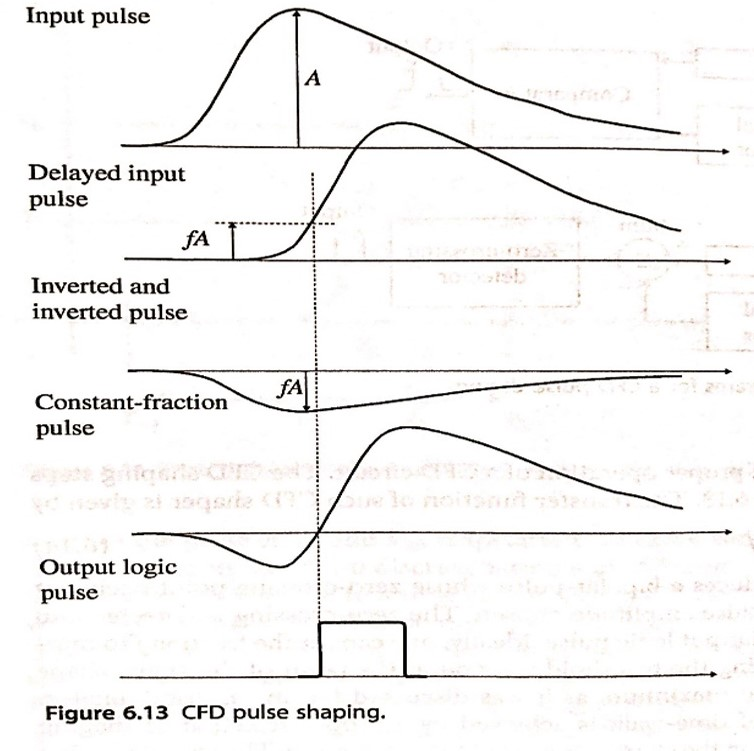
\includegraphics[width=.8\textwidth]{figures/chapter3_TDC/cfd.jpg}
\caption{Schematic of the principle of CFD algorithm}
\label{fig:TDC_cfd}
\end{figure}
\begin{figure}[t!p]
\centering
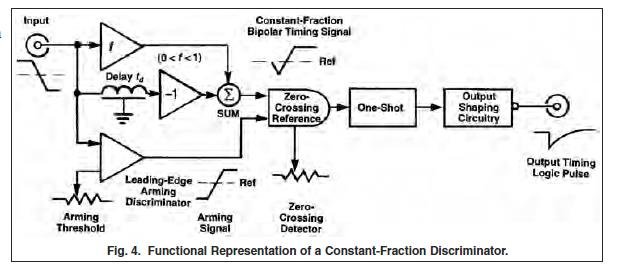
\includegraphics[width=.8\textwidth]{figures/chapter3_TDC/cfd_circuit.jpg}
\caption{Schematic of a CFD circuit}
\label{fig:TDC_cfdcircuit}
\end{figure}
The major advantage of the CFD is that it theoretically eliminates the walk error due to the independence of the zero-crossing point on pulse amplitude as shown in Figure \ref{fig:cfd_zerocrossing}. However, in practice, a finite amount of charge is required to move the comparator output from “0” to “1”, which results in additional walk error on the timing results\citep{nakhostin2017signal}. Additionally, since the summation is carried out at the peak of the signal, the traditional CFD also suffers from the saturation of the APD or multiple returns from a transmitted pulse. In other words, if the incoming signal has strong amplitude beyond the dynamic range of the photon detector which saturates the detector, or multiple returns come back in a minuscule time difference, the top of the pulse is flattened. The flattop could result in large walk error on timing results, which is why the traditional CFD is normally used in a limited range of 1:100 or less for the input signal\citep{kurtti2011integrated}\par
%, and the use of CFD less than 100: [12] [15] [26] – check ref.]}\par
\begin{figure}[t!p]
\centering
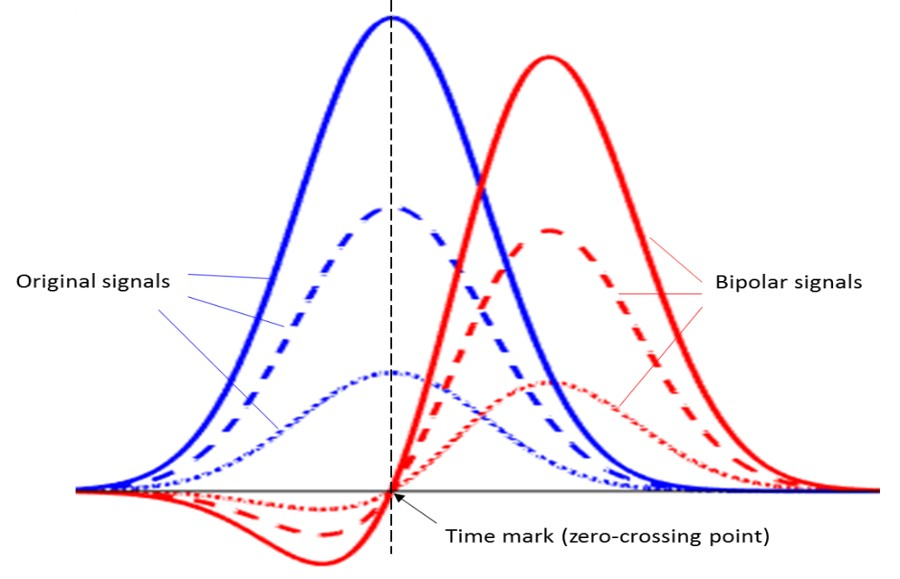
\includegraphics[width=.8\textwidth]{figures/chapter3_TDC/cfd_zerocrossing.jpg}
\caption{Independence of the zero-crossing point on signal amplitude}
\label{fig:cfd_zerocrossing}
\end{figure}
In addition to reducing the walk error, the CFD also often results in less time jitter. In principle, in the summation process of the CFD, the noises of the attenuated and the delayed signals are added as well, which should result in an increase of the variance of the noise on the bipolar signal by a factor of $1+f^2$:
$$
\sigma_{CFD}^2=(1+f^2)\sigma^2
$$
where $f$ is the CFD attenuation factor, $\sigma^2$ is the variance of the original signal, and uncorrelated noise condition is assumed [https://www.ortec-online.com/-/media/ametekortec/application\%20notes/an42.pdf]\todo{change citation}. According to Equation \eqref{eq:TDC_jitter}, the jitter for the CFD is worse compared to the leading-edge detection (of which the noise variance is sigma). However, the CFD virtually reduces the jitter, because the statistical variation of the noise on the attenuated and the delayed signals cancel out each other and consequently, the jitter is mitigated. Moreover, since only the leading edge and the peak of the signal are involved in the summation, the CFD is not limited by the pulse symmetricity. 
\subsubsection{Leading-falling edge CFD}
Noticing the limitation by involving the peak of signals, a variation of the traditional CFD, leading-falling edge CFD was developed to avoid this issue. The principle of the leading-falling edge CFD is similar to the traditional CFD as shown in Figure \ref{fig:cfd_leadFall}, which divides the original signal to two identical signals. But the rest steps are different: no signal is attenuated, but one of the signals is delayed by a certain amount, such that the leading edge of the delayed pulse and the falling edge of the non-delayed pulse cross at the optimal constant fraction of the signal height. In this case, the two signals are intersected at rather than the peak but a fraction point which has the largest slew rate of the signal. The leading-fall edge CFD can prevent the detection suffering from the flattops, but since the technique involves the falling edge of the signal, it is only practical for symmetric pulses. 
\begin{figure}[t!p]
\centering
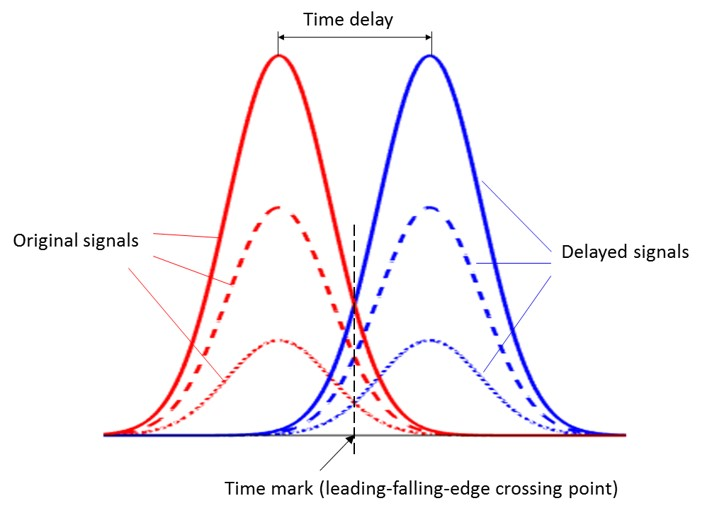
\includegraphics[width=.8\textwidth]{figures/chapter3_TDC/cfd_leadFall.jpg}
\caption{Principle of leading-falling edge CFD}
\label{fig:cfd_leadFall}
\end{figure}
\subsection{Summary}
From the comparison of the leading-edge and CFD detection, we can see that leading-edge detections have a simpler circuit design than the CFD techniques which need delay and summation circuits, but the walk error is a major drawback for the leading-edge discrimination techniques. Therefore, additional compensation techniques that are operative in a large dynamic range are required to achieve high timing accuracy. On the other hand, the CFD techniques provide a solution to significantly address the walk error and jitter, but potential time delay could result from the extra electrical components. The limited operative range of the CFD techniques also restrains their application in the automotive industry.
%%
% ADC
%%
\section{ADC-based Time Discrimination}
% Trigger Modes edge and level triggers 
\subsection{Digital Processing}
The ADC-based time discrimination is using ADC to convert analog signals output from a detector to digital signals, and measure the time of the digital returning pulse. The structure of the ADC-based discriminator is shown in Figure \ref{fig:schematic_ADC}.\par 
The digitization process of an ADC consists of two steps: sampling and quantization. The sampling step is to sample the analog signal in time by a sample-and-hold device that takes and holds a value from the continuous signal every $T_s$ second. The time interval $T_s$ is called the sampling interval and the sampling rate is denoted as $f_s$ = $1/T_s$. The resultant signal has a discrete time sequence but still continuous values for amplitude. In the quantization step, the continuous amplitude is converted to discrete values by a quantizer, and subsequently, a signal with discrete values in both time and amplitude, the so-called digital signal, is generated and output from the ADC.
\begin{figure}
\centering
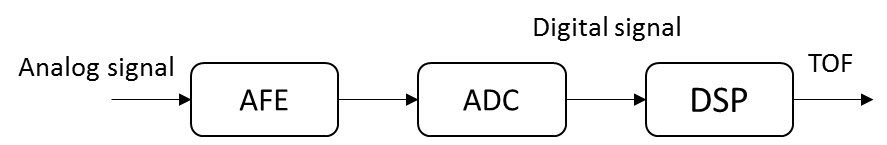
\includegraphics[width=.8\textwidth]{figures/chapter3_TDC/ADC_schematic.jpg}
\caption{Schematic of ADC}
\label{fig:schematic_ADC}
\end{figure}
\subsection{Quantization}
In the quantization process, an important parameter of the quantizer is the resolution, which indicates the number of discrete values (quantization levels) it can produce over the dynamic range of the signal amplitude. The resolution is usually expressed in bits. For example, for a 6 bits ADC, there are $2^6$ discrete values or levels to store the signal amplitude. The difference between two successive quantization levels is called quantization steps \citep{nakhostin2017signal}
\begin{align}
\Delta = V_{k+1} – V_k 
\end{align}
Thus, the quantization steps Delta and the ADC resolution B, are related to the range R of the input signal:
\begin{align}
R=2^B\Delta    
\end{align}
As seen above, the nature of the quantization process is to approximate the continuous signal by discrete values. Thus, the finite number of quantization levels introduces error between the digital signal and the original analog signal. The error is denoted as the quantization error, and it is a function of the quantization step:
\begin{align} \label{eq:ADC_quanError}
\delta^2=\frac{\Delta^2}{12}     
\end{align}
where sigma is the standard deviation of the quantization error. The signal-to-quantization noise ratio  defined as the ratio of the signal power to the noise power, can be written in dB as \citep{nakhostin2017signal}
\begin{align} \label{eq:ADC_snrDB}
SNR_{dB} = 6.02B + 1.76    
\end{align}. It should be noticed that an ADC with high resolution would have less quantization error and a large signal SQNR.
\subsection{Sampling and aliasing}
The sampling rate of the ADC also affects the reconstruction of the analog signal. As known from the Nyquist’s theorem, the sampling rate should be equal to or larger than twice the largest frequency (Nyquist frequency) of the signal to correctly represent the signal, i.e.$ f_s \geqslant 2f_{max}$. Otherwise, aliasing occurs. However, it is not always possible to precisely measure the bandwidth of the input signal of the ADC, so the Nyquist criterion may not be met in practice. Therefore, to prevent aliasing, a low-pass filter is usually placed before the ADC (the AFE shown in Figure 10), to remove or attenuate the frequency components larger than the Nyquist frequency, and such filter is called anti-aliasing filter. In many cases, the anti-aliasing filter cannot completely remove all the high-frequency components due to the transition band of the analog filter. Therefore, to minimize the aliasing, an anti-aliasing filter could be designed to attenuate the frequency higher than the Nyquist frequency to a degree less than the quantization error\citep{mitra2006digital}. This could be achieved by selecting a filter with a sharp transition band or sacrificing some in-band frequencies by moving the transition band inside the bandwidth. However, either sharp transition band or cutting off in-band frequencies could cause distortion of the original signal. Alternatively, oversampling of the signal to a rate much higher than the Nyquist frequency is also often used to simplify the anti-aliasing filter and reduce the aliasing error.
\subsection{Functionality of an ADC}
Important functionality of an AD is introduced next, and the first one is the ADC mode. An ADC usually has multiple channels taking analog inputs, and the channels share one ore more that one clocks. The ADC mode is the combination of the channels that can be used. Taking a 4-channel ADC (Channel A, B, C, D) with a clock (5GHz) as an example, the ADC can be operated in 1-channel(Channel A, B, C, D), 2-channel(\eg AC, BD, \etc) and 4-channel mode(\eg AAAA, ABCD, \etc). Since all the channels share one clock, 4-channel mode has sampling frequency of 1.25GHz signal, one forth of the speed of 1-channel mode (5GHz). In the application of TOF estimation, the 2-channel mode is used which takes the analog signals from the laser source (START signal) and the photon-detector(STOP signal) as the inputs. Another feature of an ADC is the analog offset. Using the analog offset function, users can remove the DC of the signal to maintain the signal in the middle of the ADC range, which maximizes the dynamic range.\par
The zero-suppression function is also important for an ADC to reduce the load of data transfer. The zero suppression means only the ADC only start to acquire data when the predefined ADC threshold are exceed, and the stored waveform data is referred as 'packets'. A packet contains the sampled data and the absolute time of the last sample of the packet, and the absolute time is measured since the data acquisition start. Additionally, the ADC can also save a number of samples before the ADC trigger point, which is call precursor. The timestamp of each sample of a signal have to be calculated using the time interval between the successive samples and the number of samples. Moreover, the zero suppression function have two trigger modes: edge-triggering and level triggering, which collect data in two different ways. The two trigger modes acquire data in the unit of bin, which is a group of 8 points for 2-channel mode. The edge-trigger mode specifies the length of the precursor in bins and the number of bins after the ADC trigger point (collection length), which means all the data collected under the edge-trigger mode has the same length, but not all the samples are guaranteed to be above the threshold . On the contrary, the level-trigger mode saves all the samples above the threshold instead of saving a fixed number of samples, which means the length of the stored data is dependent on the signal. In addition, the level-trigger mode can not only save samples before the trigger point, but also save samples after the point becomes lower than the threshold, which is call post-cursor. The edge and level trigger mode are illustrated in Figure~\ref{fig:ADC_edge} and Figure~\ref{fig:ADC_level} \todo{change schematic of level and edge trigger, add label of precursor and post cursor, change the context using after-cursor to postcursor}
\begin{figure}[t!p]
\centering
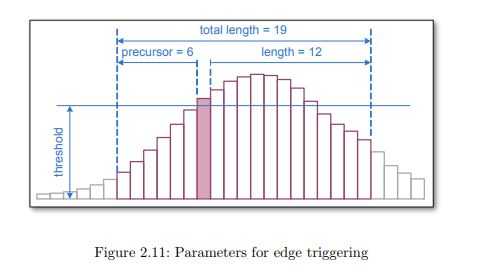
\includegraphics[width=1\textwidth]{figures/chapter_background/ADC_edge.jpg}
\caption{Edge-trigger mode}
\label{fig:ADC_edge}
\end{figure}
 
\begin{figure}[t!p] 
\centering
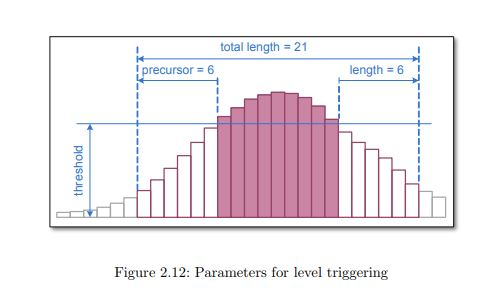
\includegraphics[width=1\textwidth]{figures/chapter_background/ADC_level.jpg}
\caption{Level-trigger mode}
\label{fig:ADC_level}
\end{figure}
 